% Definition of the radii
\def\firstradius{(0,0) circle (1.5cm)}
\def\secondradius{(0:2cm) circle (1.5cm)}
\def\scale{0.85}

\colorlet{circle edge}{black!50}
\colorlet{circle area}{gray!20}

\tikzset{
  filled/.style={fill=circle area, draw=circle edge, thick},
  outline/.style={draw=circle edge, thick}
  }

\setlength{\parskip}{5mm}

\tikzstyle{edge} = [draw, thick,-]
\tikzstyle{vertex}=[circle,fill=black!25,minimum size=10pt,inner sep=0pt]
 
\subfloat[Initial state]{\label{fig:graphTop1}
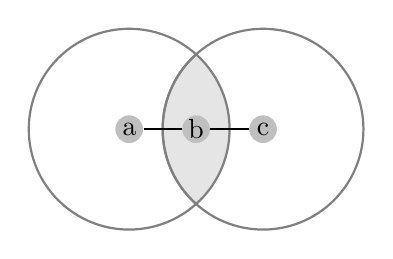
\begin{tikzpicture}[scale=\scale]
   \node[vertex] (a) at (0,0) {a};   
   \node[vertex] (c) at (2,0) {c};    

   \begin{scope}
        \clip \firstradius;
        \fill[filled] \secondradius;
    \end{scope}
    
    % Has to be defined here, or it will be overwritten 
    \node[vertex] (b) at (1,0) {b};   
 
    \draw[outline] \firstradius node {};
    \draw[outline] \secondradius node {};
    
    \path[edge] (a) -- (b);
    \path[edge] (b) -- (c);
\end{tikzpicture}}
% Remove empty line
\subfloat[Geometrical movement]{\label{fig:graphTop2}
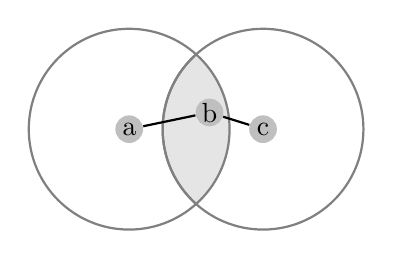
\begin{tikzpicture}[scale=\scale]
   \node[vertex] (a) at (0,0) {a};   
   \node[vertex] (c) at (2,0) {c};    

   \begin{scope}
        \clip \firstradius;
        \fill[filled] \secondradius;
    \end{scope}
    
    % Has to be defined here, or it will be overwritten 
    \node[vertex] (b) at (1.2,0.25) {b};   
 
    \draw[outline] \firstradius node {};
    \draw[outline] \secondradius node {};
    
    \path[edge] (a) -- (b);
    \path[edge] (b) -- (c);
\end{tikzpicture}
}
% Remove empty line
\subfloat[Topological movement]{\label{fig:graphTop3}
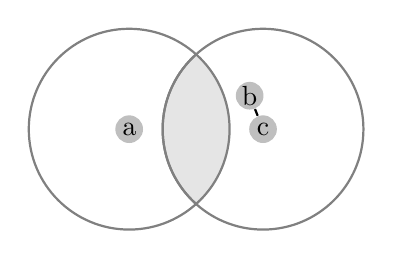
\begin{tikzpicture}[scale=\scale]
   \node[vertex] (a) at (0,0) {a};   
   \node[vertex] (c) at (2,0) {c};    

   \begin{scope}
        \clip \firstradius;
        \fill[filled] \secondradius;
    \end{scope}
    
    % Has to be defined here, or it will be overwritten 
    \node[vertex] (b) at (1.8,0.5) {b};   
 
    \draw[outline] \firstradius node {};
    \draw[outline] \secondradius node {};
    
    \path[edge] (b) -- (c);
\end{tikzpicture}
}
